%this file contains information on self-grown h-BN on the comercially bought copper foils
Copper foils with \SI{0.25}{\mm} were bought and repeatedly sputtered/annealed. Several grow cycles of h-BN via CVD of borazine were done.  The sample is transfered to the XPS-STM chamber and again sputtered/annealed serveral times to clean it properly.

The needed dosage of borazine to assemble a full monolayer of h-BN is derived via a combinated STM/XPS measurement. Several preparations were done to understand the growth behaviour of h-BN on the copper foil. Coverages are measured in STM while the chemical composition of the sample was assessed with XPS.
\begin{table}[h!]
\centering
\caption{Determination of the full monolayer borazine dosage. First a certainly saturated sample was prepared (I) and measured in XPS/STM. A sub-monolayer (II) was grown and compared to the monolayer STM and XPS results.}
 \begin{tabular}{cccccccc}
  & Prep. & Position    & Area [arb.u.] & FWHM  & Anode & Dosage  & Coverage\\ 
  &	  &	[eV]	& (XPS)		&[eV]	&Element&[L]	  & (STM) \\ \hline \hline
  \multirow{2}{*}{B1s} 	&I& 191.1 & 3776 & 1.35 & Mg & 4736 & \SI{100}{\percent}\\
    			&II& 191.1 & 1994 & 1.35 & Mg & 789 &\SI{53}{\percent}\\ \hline
  \multirow{2}{*}{N1s} 	&I& 398.7 & 5875 & 1.45 & Al  & 4736 & \SI{100}{\percent}\\
 			&II& 398.6 & 3183 & 1.43 & Al & 789 &\SI{54}{\percent}\\
 \end{tabular}
\end{table}

\begin{figure}[ht]
\centering
\subfigure[N1s]{
   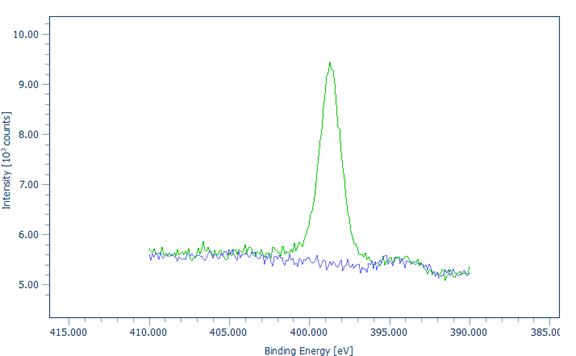
\includegraphics[width=.45\textwidth]{./images/XPS-150314-N1s.jpg}
   }
\subfigure[B1s]{
   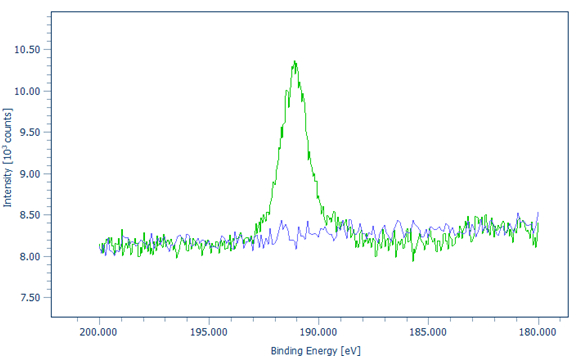
\includegraphics[width=.45\textwidth]{./images/XPS-150314-B1s.jpg}
   }
\subfigure[C1s]{
   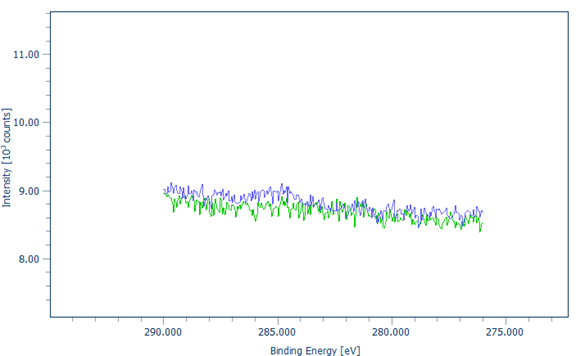
\includegraphics[width=.45\textwidth]{./images/XPS-150314-C1s.jpg}
   }
\subfigure[Cu3s]{
   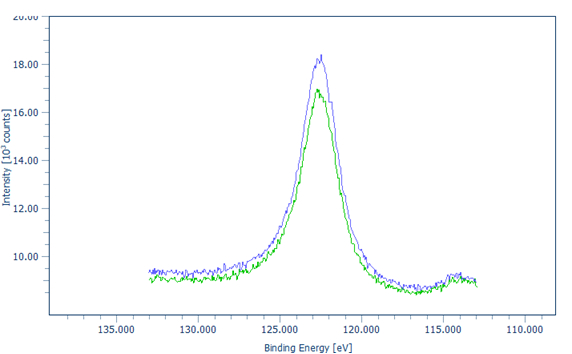
\includegraphics[width=.45\textwidth]{./images/XPS-150314-Cu3s.jpg}
   }
\caption{XPS spectra for ML h-BN/Cu-foil. The peaks are at their expected positions\cite{kidambi_situ_2014} and show no additional features. No remnants of sulfur or remaining oxygen could be found.}
\label{fig:xps-self-grown}
\end{figure}

When comparing the resulting coverage (STM coverage/XPS signal) (II) to the (saturated) monolayer (I) one can derive the minimal amount of borazine needed to process a monolayer of h-BN on the copper foil. Comparing the coverages of a sample grown with CVD, \SI{7E-6}{\milli \bar} for 15min (I) and one grown with CVD, \SI{3.5E-6}{\milli \bar} for 5min (II), shows that reducing the dosage by a factor of 6 does not reduce the coverage by a factor of 6, but just by a factor of 2. Therefore (I) features a full monolayer and (II) only half of it. It follows that a full monolayer may be achieved by dosing 1500\,L borazine on a \SI{800}{\degreeCelsius} hot copper foil surface. 
Because the growth rate may certainly not be linear (less and less free copper surface to decompose borazine into building fragments while the layer assembles) the given dosage is a minimum estimation to achieve the monolayer.

Even though a much larger amount for borazine (4736 L\,) than needed for a monolayer (1500 L\,) has been dosed, the maximum coverage did not exeed ne XPS signal of a monolayer. So the growth of h-BN on copper foil is self-limited (as in the case of many h-BN/metal systems) to a full monolayer. It is not possible to achieve layer growth with this type of preparation.

T and t dependence is not subject to investigation because the growth is supposed to follow the same mechanisms as on the single-crystal case. Quiet some investigation has been done, \cite{orlando_epitaxial_2012,preobrajenski_monolayer_2007-1} to understand this process and literature has matured.